\section{Техническое задание}

\subsection{Основание для разработки}

Основанием для разработки является задание на выпускную квалификационную работу бакалавра <<Приложение для составления тренировочного плана и отслеживания прогресса>>.

\subsection{Цель и назначение разработки}

Основной задачей выпускной квалификационной работы является разработка и тестирование программно-информационной системы для индивидуального планирования тренировок и отслеживания прогресса.

Целью разработки является создание работоспособного многопользовательского веб-приложения, позволяющего составлять и выполнять персональные планы тренировок, фиксировать результаты и распределение нагрузки по группам мышц, вести дневник питания с учётом калорийности и КБЖУ, а также поддерживать мотивацию за счёт модуля психологической поддержки, аватара с системой опыта и элементов социального взаимодействия.

Задачами данной разработки являются:
\begin{itemize}
	\item изучение предметной области и сопоставление архитектурных подходов для веб-приложений с учётом требований к хранению персональных данных и синхронизации между устройствами;
	\item проектирование программной системы;
	\item проектирование интерфейса пользователя;
	\item реализация аутентификации и управления профилем;
	\item реализация модуля тренировок;
	\item реализация модуля питания, модуля поддержки и модуля цифрового аватара;
	\item реализация социальной ленты (посты, комментарии, лайки, реакции) и клиентского модуля взаимодействия с ней;
	\item тестирование ключевых сценариев (регистрация и вход, сохранение плана и тренировки, дневник питания, публикации в ленте) и отладка взаимодействия клиента с API.
\end{itemize}

\subsection{Функциональные требования}

Ниже приведен перечень функций, которые должно обеспечивать приложение.

Аутентификация и профиль. Данный блок включает следующие возможности:
\begin{itemize}
	\item регистрация пользователя и вход в систему;
	\item управление параметрами профиля (личные данные, цели, контакты при необходимости, загрузка фотографии).
\end{itemize}

Тренировки. Приложение должно предоставлять пользователю следующие функции для работы с тренировками:
\begin{itemize}
	\item составление, редактирование и сохранение индивидуальных планов тренировок с разбиением по дням цикла;
	\item доступ к каталогу упражнений с группировкой по группам мышц и разделением силового и кардио-компонентов при планировании;
	\item использование готовых шаблонных программ;
	\item выполнение тренировки по выбранному плану и дню и фактическая фиксация результатов;
	\item ведение истории выполненных тренировок;
	\item визуальный анализ прогресса (графики, календарь, распределение нагрузки, рекомендации по нагрузке в общем виде).
\end{itemize}

Питание и КБЖУ. Для отслеживания питания предусмотрены следующие возможности:
\begin{itemize}
	\item ведение дневника приёмов пищи с привязкой к календарной дате;
	\item ручной ввод продуктов и блюд, в том числе пользовательских;
	\item расчёт и отображение калорийности и КБЖУ за день, сводок и диаграмм динамики;
	\item доступ к справочнику продуктов с поиском и выбором позиций.
\end{itemize}

Модули поддержки, аватар и дополнительная мотивация. В приложении также реализованы:
\begin{itemize}
	\item раздел поддержки пользователя с вспомогательными материалами и чекинами;
	\item модуль «Аватар» (цифровой персонаж, уровень и отображение активности).
\end{itemize}

Социальное взаимодействие. Для общения и обмена опытом между пользователями предназначены:
\begin{itemize}
	\item общая лента сообщений пользователей установки приложения с публикациями, комментариями и реакциями;
	\item поиск и упорядочивание сообщений для удобства просмотра;
	\item использование профильных данных (в т.ч. изображений) для отображения участников при обмене сообщениями.
\end{itemize}

\subsection{Роли пользователей}

До успешной аутентификации пользователь работает с экраном входа и регистрации. После входа открывается основной интерфейс с сохранением данных на сервере. Условно выделяются две роли.

Неавторизованный пользователь. Видит экран входа и регистрации.

Зарегистрированный пользователь. После входа получает полный доступ к функциям клиента: планы и журнал тренировок, питание, профиль, поддержка, аватар, социальная лента, сохранение и синхронизация данных учётной записи между сеансами работы.

Роль назначается автоматически после успешной регистрации или входа.

\subsection{Требования к интерфейсу}

Интерфейс реализуется как одностраничное приложение в браузере: до аутентификации доступен только экран входа и регистрации; после входа отображается единый каркас с постоянной верхней панелью и областью контента выбранного раздела. Переключение модулей выполняется без перезагрузки документа (кроме принудительной перезагрузки после регистрации в реализации клиента). Для иллюстрации структуры в документе используются два макета: экран авторизации и развёртка главного окна на примере модуля <<Тренировки>> (рисунки~\ref{fig:tzuiauthorization} и~\ref{fig:tzuitraining}).

\subsubsection{Экран авторизации и регистрации}

До входа пользователь видит карточку с заголовком и кратким пояснением назначения входа. Предусмотрено переключение двух режимов вкладками: <<Вход>> и <<Регистрация>>; активная вкладка визуально выделена. В режиме <<Вход>> (рисунок~\ref{fig:tzuiauthorization}) показываются поля <<Логин>> и <<Пароль>> и кнопка подтверждения (<<Войти>>). В режиме <<Регистрация>> дополнительно отображаются фамилия, имя, дата рождения (маска ДД.ММ.ГГГГ), выбор пола двумя кнопками. Сообщения об ошибках валидации и ответа сервера выводятся в той же карточке. Оформление согласовано с цветовой темой приложения.

\begin{figure}[H]
	\centering
	
\includegraphics[width=0.82\linewidth]{tz_ui_authorization.png}
	\caption{Макет экрана авторизации (режим <<Вход>>)}
	\label{fig:tzuiauthorization}
\end{figure}

\subsubsection{Главное окно: верхняя панель и пример раздела <<Тренировки>>}

После входа в верхней части экрана отображается навигационная панель (на макете рисунок~\ref{fig:tzuitraining}): переключатели пяти разделов -- <<Тренировки>>, <<Питание>>, <<Социальные сети>>, <<Поддержка>>, <<Аватар>> -- и блок учётной записи (логин, значок пользователя, вызов профиля, смена светлой\,/\,тёмной темы, выход). Активный раздел подчёркивается относительно остальных. На приведённом макете выбран раздел <<Тренировки>>; та же панель используется для перехода к остальным модулям, заменяя только содержимое рабочей области.

В колонках под панелью раскрывается функциональность <<Тренировки>>. Слева -- <<Мои планы>>, каталог упражнений по группам мышц, шаблоны программ, сводка по текущему плану и числу упражнений; внизу допускаются подсказки о серверном сохранении, теме оформления и графиках прогресса. В центре -- выбранный день плана со списком упражнений (название, группа мышц), поиск по упражнениям дня, добавление упражнения, запуск выполнения тренировки, привязка типа нагрузки, переход к графику по упражнению, удаление позиции. Справа -- аналитика: переключение <<Прогресс>>\,/\,<<Календарь>>, график нагрузки по группам мышц, блок рекомендаций по прогрессии. Компоновка поддерживает цепочку планирование -- выполнение -- анализ; при ограничении высоты окна допускается вертикальная прокрутка блоков.

\begin{figure}[H]
	\centering
	
\includegraphics[width=0.95\linewidth]{tz_ui_training.png}
	\caption{Макет главного окна: панель разделов и интерфейс модуля <<Тренировки>>}
	\label{fig:tzuitraining}
\end{figure}

\subsubsection{Разделы <<Питание>>, <<Социальные сети>>, <<Поддержка>>, <<Аватар>> и профиль}

Пункты <<Питание>>, <<Социальные сети>>, <<Поддержка>> и <<Аватар>> открываются с верхней панели (см. переключатели на рисунке~\ref{fig:tzuitraining}); иллюстрация содержимого этих модулей в настоящем разделе не приводится -- в рабочей области отображаются специализированные экраны. В <<Питание>> -- дневник приёмов на дату, приёмы со сворачиванием, поиск и выбор продуктов, показатели калорийности и КБЖУ, при необходимости график по дням. В <<Социальные сети>> -- лента постов, ввод публикаций и комментариев, элементы реакций. В <<Поддержка>> -- советы, чекины, опциональный календарь состояний и вспомогательные материалы. В <<Аватар>> -- цифровой персонаж, уровень и метрики активности. Профиль пользователя и загрузка фотографии доступны из элементов учётной записи на панели; в профиле задаются дополнительные личные данные.

\subsection{Сценарии использования}

Для наглядного представления типовых действий пользователей по ролям на рисунке~\ref{fig:diagramm} приведены диаграммы вариантов использования для неавторизованного и авторизованного пользователей соответственно.

\begin{figure}[H]
	\centering
	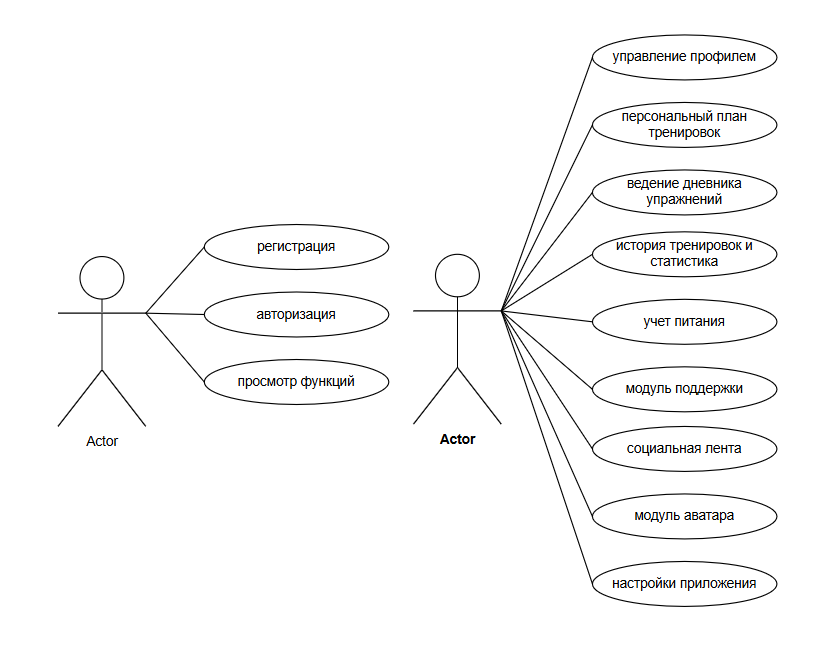
\includegraphics[width=0.90\linewidth]{images/diagramm.png}
	\caption{Диаграммы вариантов использования}
	\label{fig:diagramm}
\end{figure}

\subsubsection{Регистрация нового пользователя}

Пользователь открывает приложение и попадает на экран входа. Для создания новой учётной записи переключается на вкладку <<Регистрация>>, после чего на экране появляется расширенный набор полей: помимо имени входа и пароля система предлагает указать фамилию, имя, дату рождения и пол. Заполнив необходимые поля, человек отправляет регистрационную анкету.

Система проверяет, что информация представлена в допустимом виде: что обязательные поля не пустые, что дата рождения выглядит корректно, что логин и пароль удовлетворяют простым ограничениям по минимальной длине или формату, принятым в приложении. Если уже существует пользователь с таким же именем входа, об этом сообщают понятным текстом, чтобы человек мог выбрать другое имя входа или войти под существующей учётной записью.

При успешной регистрации пользователь становится авторизованным: открывается основное окно приложения с разделами тренировок, питания, социальной активности и прочего функционала. Часть сведений, не обязательных при первоначальной анкете, человек имеет возможность добавить позже в профиле, когда будет удобно.

\subsubsection{Вход в систему}

Пользователь, ранее прошедший регистрацию, выбирает вкладку <<Вход>>, вводит своё имя входа и пароль и подтверждает действие.

Если имя входа и пароль соответствуют ранее зарегистрированной учётной записи этого пользователя, система показывает главный интерфейс с сохранёнными его данными.

Если вход не удался -- например из-за неверного пароля -- приложение сообщает об этом без раскрытия лишних деталей, чтобы исключить злоупотребления со стороны посторонних, и пользователь может повторить ввод или воспользоваться регистрацией, если учётную запись ещё не создавал.

\subsubsection{Заполнение и изменение профиля}

Из основного интерфейса пользователь переходит к разделу личной учётной записи и открывает экран профиля. Здесь он может уточнить или изменить параметры тела и целей, добавить текстовые пояснения о фитнес-задаче и уровне активности, при необходимости указать город, контактные данные или краткие медицинские заметки, которые сам считает уместными хранить в приложении для собственной ориентации. Допускается загрузка фотографии для отображения в интерфейсе.

После сохранения изменений система показывает обновлённые данные там, где профиль представлен пользователю и там, где визуально обозначаются участники в других частях приложения -- например в социальной ленте. Если какие-либо значения указаны недопустимо или сохранить их не удалось, пользователь получает понятное сообщение и может поправить анкету.

\subsubsection{Создание и корректировка индивидуального плана тренировок}

Пользователь переходит в раздел <<Тренировки>> и находит блок со своими сохранёнными планами. Он может начать новый цикл занятий <<с чистого листа>>, задав собственное имя плана и число тренировочных дней в недельном\,/\,циклическом режиме, либо взять готовый шаблон программы как отправную точку и затем отредактировать её под себя.

Далее из каталога упражнений, сгруппированного по области тела\,/\,мышечным группам и типу нагрузки, пользователь переносит нужные упражнения на выбранные дни. Для каждой позиции задаёт запланированное число подходов, повторений и\,/\,или рабочий вес, при необходимости переименовывает или дублирует целый день\,/\,фрагмент плана для ускорения настройки. Готовое расписание сохраняется под выбранным именем.

Система отображает план в общем списке, позволяет переключаться между сохранёнными вариантами, открыть конкретный день перед тренировкой и при необходимости вернуться к редактированию: добавить упражнение, удалить позицию, изменить параметры без потери уже накопленной истории по другим занятиям.

\subsubsection{Выполнение тренировки по плану}

Перед началом занятий пользователь указывает, каким планом он пользуется и какой это день в цикле. На экране появляется список запланированных упражнений с ориентирами по подходам.

В ходе тренировки человек выполняет подходы и фиксирует факт: реальное число повторений, массу отягощения или иные показатели, которые поддерживаются интерфейсом для данного типа упражнения. Система по возможности подсказывает значения из прошлых успешных тренировок, чтобы не вводить одно и то же заново.

По окончании серии упражнений пользователь явно завершает занятие. Тогда приложение считает день выполненным, заносит сведения в журнал тренировок и обновляет все экраны, где отображается прогресс: графики, календарь, суммарные показатели. Дополнительно накопление регулярных занятий может отображаться через модуль мотивации с цифровым аватаром.

\subsubsection{Ведение дневника питания}

В разделе <<Питание>> пользователь указывает интересующий календарный день -- например текущее число -- чтобы вести дневник строго <<за сегодня>> или просмотреть\,/\,дополнить прошлые даты.

Внутри суток добавляются отдельные приёмы пищи: завтрак, обед, перекуски -- названия и число блоков зависят от привычек пользователя. В каждый блок помещаются позиции: либо выбранный из приложенного справочника продукт или блюдо, либо собственное описание с приблизительной порцией, если нужной записи ещё нет.

Приложение суммирует калорийность и долю белков, жиров и углеводов по дню, показывает итог в компактном виде и может нарисовать тенденцию за несколько дней подряд, чтобы человек видел общую картину, а не только одну строку счёта. Приём пищи можно сворачивать после заполнения, чтобы не засорять экран во время активного расчёта рациона.

\subsubsection{Раздел поддержки и отметки самочувствия}

Открывая раздел <<Поддержка>>, пользователь получает доступ к текстовым советам, подсказкам по восстановлению и регулярности тренировок, а также к простым действиям вроде чекина за день: отметить настроение, отметить факт тренировки или отдыха. Это необязательный сценарий, но если человек его использует, система сохраняет записи как личную хронику и может показывать их только ему же при последующих визитах.

\subsubsection{Модуль <<Аватар>> и наблюдение за <<опытом>>}

Пользователь переключается на раздел <<Аватар>>, где видит оформленного персонажа -- иллюстративную <<награду>> за регулярность и объём нагрузок. По мере сохранённых и завершённых тренировок уровень или стадия персонажа обновляется; приложение сообщает это ненавязчиво через визуальные изменения и краткие подписи, без превращения модуля в отдельную игру. Человек может заглянуть туда перед или после недели занятий, чтобы зафиксировать ощущение прогресса.

\subsubsection{Активность в социальной ленте}

В разделе <<Социальные сети>> перед пользователем открыта общая для данной установки приложения лента публикаций. Он может прочитать записи других зарегистрированных участников с их именами входа\,/\,никами\,/\,маленькими изображениями профилей, переходить к комментированию тем, которые его заинтересовали.

Собственную мысль о тренировке, результате\,/\,переживании пользователь может оформить как новый пост после ввода текста в предназначенной для этого области. Если лента длинная, для удобства предусмотрены поиск по словам и упорядочивание сообщений -- например сначала самые новые или наоборот старые, в зависимости от режима интерфейса.

Оценивая содержание, человек ставит символический <<лайк>>, выбирает эмодзи-реакцию среди набора приложения или оставляет ответ в виде цепочки комментариев под постом. Если какие-то авторы кажутся полезнее остальных, пользователь может отметить их внутри приложения как приоритетных для быстрой фильтрации при следующих визитах. Автор имеет возможность временно закрепить свой пост над лентой, если такая возможность поддерживается в интерфейсе.

Система отражает результат действий человека сразу в ленте: новый пост, обновившийся список реакций, новый порядок при смене сортировки. Запрещённые или недопустимые по правилам приложения сообщения приложение не должно добавлять; при технических сбоях пользователь получает предупреждение о неудаче операции без потери уже введённого текста, где это возможно.

\subsubsection{Просмотр статистики и истории результатов}

Пользователь возвращается в раздел <<Тренировки>> или использует уже знакомые панели анализа и там выбирает интересующий показатель: конкретное упражнение для просмотра динамики силового результата, сводную диаграмму распределения нагрузки по группам мышц, календарь с отмеченными завершёнными днями. Это позволяет ответить на вопросы <<что уже работает>>, <<равномерно ли распределены нагрузки>>, <<как часто в последнее время выполняются планы>>.

При необходимости для мотивации человек дополнительно открывает <<Аватар>> и видит связку между наблюдаемым прогрессом в числах и наглядной <<выдачей>> персонажа. Отдельным запросом к питательному журналу тот же человек может сопоставить графики тренировочной активности и динамику калорийности за неделю, если оба режима заполняются регулярно -- приложение просто параллельно хранит и показывает эти два контура данных.

\subsection{Требования к оформлению документации}

Разработка программной документации и программного изделия должна производиться согласно ГОСТ~19.102-77 и ГОСТ~34.601-90. Единая система программной документации.
